\documentclass[11pt]{article}

\usepackage[utf8]{inputenc}
\usepackage[margin=1in]{geometry}
\usepackage{amsmath,amssymb}
\usepackage{graphicx}
\usepackage{natbib}
\usepackage{hyperref}
\usepackage{booktabs}
\usepackage{xcolor}
\usepackage{setspace}
\onehalfspacing

\title{Forward Flux Sampling for Rare Atmospheric Events: Bridging Statistical Mechanics and Neural Weather Emulation}

\author{%
  John S. Schreck$^{1,*}$ \\
  \small $^1$National Center for Atmospheric Research, Boulder, CO \\
  \small $^*$Corresponding author: schreck@ucar.edu
}

\date{\today}

\begin{document}

\maketitle

\begin{abstract}
Tropical cyclogenesis, extreme heatwaves, and rapid intensification events are rare atmospheric phenomena that pose significant forecasting challenges. Their infrequent occurrence and the computational expense of generating sufficient statistics through direct ensemble sampling make probabilistic prediction difficult. We demonstrate that Forward Flux Sampling (FFS), a path sampling technique originally developed for molecular rare events, can be successfully adapted to study tropical cyclone genesis in neural weather emulators. Unlike equilibrium-based approaches, FFS requires no assumptions about detailed balance or free energy landscapes, making it particularly well-suited to the non-equilibrium steady state (NESS) dynamics of the atmosphere. We frame rare atmospheric events as transitions between regions of a strange attractor in high-dimensional phase space, where genesis occurs through dynamical alignment of environmental conditions rather than thermal fluctuations over energy barriers. Using a learned atmospheric model (SDL-WXFormer) trained on ERA5 reanalysis, we implement FFS with minimum sea-level pressure as an order parameter, augmented by Cyclone Phase Space thermal structure analysis to distinguish tropical from extratropical systems. Applied to 18 Atlantic basin initial conditions from August--September 2022, FFS achieves 20--30 percent statistical uncertainty in genesis rate estimates using approximately 25 GPU-hours per initial condition, compared to 400+ GPU-hours required for equivalent direct ensemble sampling. Enhancement factors range from 10 to 50 depending on atmospheric regime and genesis probability. This work establishes a methodological bridge between computational statistical mechanics and atmospheric science, demonstrating that non-equilibrium rare event sampling techniques enable systematic study of extreme events in both physics-based and machine learning weather models.
\end{abstract}

\section{Introduction}

\subsection{The Challenge of Atmospheric Rare Events}

Tropical cyclone genesis represents a fundamental challenge in probabilistic weather prediction. Observational climatologies indicate that approximately 10 to 15 percent of tropical waves and disturbances develop into named systems \citep{Frank1970,Landsea1998}, but discriminating viable precursors from non-developing cases continues to challenge deterministic and ensemble forecasting approaches \citep{Titley2019,Halperin2013}. A tropical cyclone forming in the Atlantic basin occurs with probability $\sim 10^{-3}$ per day for a given atmospheric state during peak season, yet approximately 12 such events occur annually. Accurately predicting which disturbances will undergo genesis requires understanding transition pathways through high-dimensional atmospheric phase space. These pathways are rarely traversed in direct numerical simulations.

The computational challenge is fundamental. A state-of-the-art ensemble prediction system might run 50 members for 10 days, sampling 500 days of atmospheric evolution. For a rare event with probability $10^{-4}$ per day, this ensemble would be expected to capture zero events through direct sampling. Achieving statistically meaningful uncertainty bounds requires observing sufficient successful genesis events, necessitating ensemble sizes that far exceed current computational feasibility. For genesis probability $p \sim 10^{-3}$ and target relative uncertainty of 20 percent, direct Monte Carlo estimation requires approximately 25 successful observations, implying ensemble sizes of $\sim 25,000$ members per initial condition. At computational costs of approximately 1 GPU-minute per 10-day forecast at operational resolution, systematic climatological analysis across multiple atmospheric regimes becomes infeasible.

Climate modeling faces analogous challenges. Projecting changes in tropical cyclone frequency under greenhouse warming requires multi-millennial integrations at convection-permitting resolution. This computational burden remains prohibitive. Rare event sampling techniques offer an alternative by concentrating computational effort on transition pathways rather than basin residence times. We can thus estimate rates of events that would never be observed in direct simulation.

\subsection{Rare Event Sampling in Statistical Mechanics}

The molecular simulation community confronted similar challenges decades ago. Processes such as protein folding, crystal nucleation, and chemical reactions involve transitions between metastable states separated by free energy barriers. Waiting times between transitions ($\sim 10^{-3}$ to $10^6$ seconds) vastly exceed accessible molecular dynamics timesteps ($\sim 10^{-15}$ seconds), creating a computational gap of 10-20 orders of magnitude.

This timescale separation motivated development of specialized sampling techniques. Transition Path Sampling \citep{bolhuis2002transition} generates ensembles of reactive trajectories by Monte Carlo moves in path space. Metadynamics \citep{laio2002escaping} accelerates barrier crossing through history-dependent biasing potentials. Forward Flux Sampling \citep{allen2006forward,allen2009forward}, the focus of this work, uses a series of interfaces between initial and final states to compute transition rates without modifying the underlying dynamics.

The theoretical foundation of these methods rests on equilibrium statistical mechanics: systems evolve according to Hamiltonian dynamics with stochastic forcing from a thermal bath, and steady-state distributions obey detailed balance. Rate constants connect to free energy differences through transition state theory. Order parameters (reaction coordinates) describe progress along a one-dimensional projection of high-dimensional configuration space.

\subsection{Extending Rare Event Theory to Atmospheric Dynamics}

Atmospheric systems differ fundamentally from molecular ensembles. The atmosphere is a driven-dissipative system maintained far from equilibrium by solar forcing and radiative cooling. No thermal bath exists at planetary scales. Stochasticity arises from unresolved turbulent cascades and parametrization uncertainty rather than Brownian motion. Detailed balance does not apply. Conventional thermodynamic concepts like free energy landscapes, partition functions, and Boltzmann distributions lack rigorous definitions for non-equilibrium continuum mechanics.

Yet the atmosphere exhibits rare events such as tropical cyclogenesis, extreme heatwaves, and sudden stratospheric warmings. These events occur infrequently not because they correspond to high-energy states unlikely under thermal fluctuations, but because atmospheric trajectories rarely visit certain regions of the system's strange attractor. The rarity is geometric and dynamical rather than energetic. This distinction suggests that rare event methods designed for non-equilibrium systems may be more appropriate for atmospheric applications than equilibrium-based techniques.

Despite these theoretical obstacles, the algorithmic machinery of rare event sampling remains applicable. Forward Flux Sampling, in particular, was designed for non-equilibrium systems and does not require equilibrium assumptions beyond Markovian dynamics \citep{allen2009forward}. The method computes flux-weighted transition probabilities through a series of interfaces, a purely kinetic quantity independent of any underlying thermodynamic structure. The atmosphere is a non-equilibrium steady state (NESS) with time-invariant statistics maintained by continuous forcing and dissipation. This is precisely the regime for which FFS was intended.

Recent applications have demonstrated this portability. \citet{ragone2018computation} applied importance sampling techniques to extreme heatwave generation in CESM, achieving 100-1000$\times$ computational efficiency gains. \citet{webber2019practical} used quantile diffusion Monte Carlo to sample intense tropical cyclone realizations in WRF. \citet{plotkin2019maximizing} employed action minimization to identify most-probable intensification pathways. These studies establish precedent for adapting statistical mechanical methods to atmospheric rare events, though all employed physics-based numerical models rather than learned emulators.

\subsection{Neural Weather Emulation and Rare Events}

Machine learning-based weather prediction has achieved remarkable progress. Models such as GraphCast \citep{lam2023graphcast}, Pangu-Weather \citep{bi2023pangu}, and FourCastNet \citep{pathak2022fourcastnet} now rival or exceed physics-based ensemble forecasts at medium-range timescales (3-10 days). These systems learn atmospheric evolution operators directly from reanalysis data, bypassing explicit discretization of governing equations.

The SDL-WXFormer architecture \citep{schreck2024sdl} extends this paradigm to ensemble forecasting through stochastic decomposition layers adapted from generative modeling \citep{karras2019stylebased}. The model learns to inject state-dependent noise that captures flow-regime-dependent predictability characteristics, generating ensemble spread calibrated to ERA5 ensemble statistics. The model operates as a learned operator $\mathcal{M}: \mathbb{R}^d \to \mathbb{R}^d$ mapping atmospheric states forward in 6-hour increments, where the mapping is encoded in neural network weights ($d \sim 10^7$ for operational resolution) rather than explicit physical equations.

For rare event applications, learned emulators offer distinct advantages: computational efficiency (1000$\times$ faster than physics models), differentiability (enabling gradient-based optimization), and natural ensemble generation (through learned stochasticity). However, they also introduce theoretical complications. The configuration space is a learned manifold rather than primitive dynamical variables. Training data may underrepresent extreme events. Extrapolation beyond training distributions raises questions about physical fidelity.

\subsection{Scope and Objectives}

This work demonstrates that Forward Flux Sampling can be successfully implemented for tropical cyclogenesis in neural weather emulators, establishing proof-of-concept for rare event sampling in learned atmospheric models. We address three primary questions:

\begin{enumerate}
    \item \textbf{Order Parameter Validity}: Can integrated macroscopic quantities (minimum sea-level pressure) serve as legitimate progress coordinates for atmospheric rare events, or does the absence of equilibrium thermodynamics invalidate concepts borrowed from molecular simulation?
    
    \item \textbf{Learned Dynamics}: How do statistical mechanical frameworks apply to neural emulators where atmospheric evolution is learned from data rather than governed by explicit conservation laws?
    
    \item \textbf{Practical Implementation}: What computational strategies enable robust FFS calculations for chaotic, spatially extended systems? This includes interface placement, trajectory termination criteria, and feature tracking.
\end{enumerate}

While we focus on tropical cyclogenesis as a concrete demonstration, the methodology generalizes immediately to other atmospheric rare events: extreme heatwaves, sudden stratospheric warmings, blocking onset, atmospheric river formation, and rapid intensification of existing cyclones. The goal is not merely to compute genesis rates for specific cases but to establish a methodological framework applicable across atmospheric science.

The remainder of this paper is organized as follows. Section 2 examines theoretical considerations for applying FFS to data-driven atmospheric models, addressing metastability, deterministic chaos, and non-equilibrium dynamics. Section 3 presents the FFS formalism including flux and conditional probability definitions with visual schematic illustration. Section 4 describes implementation details for SDL-WXFormer including order parameter specification, interface placement, and parallel algorithms. Section 5 presents results for 18 initial conditions from August--September 2022, including operational IFS ensemble baseline comparison. Section 6 discusses implications for operational probabilistic forecasting and extensions to other rare atmospheric transitions.
\section{Applicability of Forward Flux Sampling to Neural Weather Models}

\subsection{Non-Equilibrium Steady States and Atmospheric Dynamics}

The fundamental question is whether Forward Flux Sampling, developed for molecular systems obeying equilibrium statistical mechanics, can be meaningfully applied to atmospheric dynamics which manifestly do not satisfy equilibrium conditions. We argue that FFS is, in fact, \textit{more} appropriate for atmospheric rare events than equilibrium-based methods precisely because it does not require equilibrium assumptions.

The atmosphere is a canonical example of a non-equilibrium steady state (NESS). Solar forcing continuously injects energy at low latitudes and short wavelengths. Radiative cooling extracts energy at high latitudes and long wavelengths. Friction dissipates kinetic energy. The system maintains time-invariant statistical properties without ever reaching thermodynamic equilibrium. Entropy is continuously produced and exported to space. This driven-dissipative character persists across all timescales relevant to weather and climate.

Forward Flux Sampling requires no equilibrium assumption. The method needs only three ingredients \citep{allen2009forward}. These are a well-defined stochastic or chaotic dynamical system, distinguishable metastable regions in state space, and measurable flux between those regions. Detailed balance, Boltzmann distributions, free energy landscapes, and reversibility are \textit{not} required. FFS computes flux-weighted transition probabilities that are purely kinetic quantities independent of any underlying thermodynamic structure.

The key theoretical framework is that of chaotic attractors. The atmospheric state evolves on a strange attractor embedded in high-dimensional phase space. Synoptic-scale flows populate certain regions of this attractor more frequently than others, corresponding to quasi-stationary weather regimes. Rare events are transitions between different regions of the attractor. For instance, the transition from a state characterized by unorganized tropical disturbances to a state supporting an organized tropical cyclone. These are \textit{dynamical} transitions governed by the vector field of atmospheric equations, not \textit{thermodynamic} transitions governed by free energy differences.

This distinction is crucial. Equilibrium statistical mechanics describes systems that explore configuration space according to $P(x) \propto \exp(-E(x)/k_BT)$, sampling high-energy states rarely because thermal fluctuations are unlikely to overcome energy barriers. Atmospheric rare events occur not because "thermal fluctuations" are insufficient but because the deterministic flow plus stochastic forcing rarely visits certain attractor regions. A tropical cyclone is rare not because it has high "energy" but because initial conditions and environmental parameters must align in specific ways for genesis to occur. The rarity is geometric and dynamical, not energetic. Hurricanes actually release enormous amounts of stored potential energy.

Forward Flux Sampling is ideally suited to such systems. The method makes no assumptions about why certain transitions are rare. It only requires that they are rare and that one can measure fluxes through interfaces separating different regions. This makes FFS applicable to non-equilibrium steady states, time-periodic systems, and even transient regimes, provided the metastable states exist and the order parameter meaningfully distinguishes them.

\subsection{Learned Dynamics and State Propagation}

Neural weather models do not solve differential equations describing atmospheric fluid dynamics. Instead, they learn state-to-state transformations directly from historical reanalysis data through supervised training on observation-based datasets spanning decades. The SDL-WXFormer model encodes atmospheric evolution as a neural operator $\mathcal{M}: \mathbb{R}^d \to \mathbb{R}^d$ where network weights, rather than discretized physical laws, determine state propagation. Despite this fundamental difference in dynamical representation, the theoretical framework of Forward Flux Sampling applies without modification because the method requires only well-defined states, measurable transition rates, and trajectories connecting those states. The mechanism generating trajectories is irrelevant to the mathematical structure of flux and conditional probability factorization. It does not matter whether trajectories come from molecular dynamics integration, numerical weather prediction, or neural network inference.

The SDL-WXFormer architecture comprises approximately 1.5 billion parameters trained on ERA5 reanalysis spanning 1979-2021 at 6-hour temporal resolution. The model predicts 69 pressure-level variables and 8 surface variables at 1° spatial resolution (~110 km at equator). Training employed multi-step loss functions extending to 40 forecast steps (10 days), forcing the network to learn self-consistent atmospheric evolution rather than single-step state mapping. Spectral constraints preserve kinetic energy distributions across scales, ensuring mesoscale features (100-1000 km) characteristic of tropical cyclones are represented accurately.

\subsection{Metastability as Attractor Structure}

Metastability in non-equilibrium systems differs fundamentally from equilibrium metastability. In molecular systems, metastable states correspond to local minima in a free energy landscape; thermal fluctuations cause rare barrier crossings. In atmospheric dynamics, metastability arises from the geometry of the strange attractor: the system's flow concentrates probability density in certain attractor regions while infrequently visiting others.

Consider tropical cyclogenesis in the Atlantic basin during boreal summer. The atmospheric state vector evolves on a high-dimensional attractor. Most trajectories on this attractor correspond to the climatological background such as easterly waves, tropical disturbances, and synoptic-scale variability, the majority of which dissipate without intensification. This background regime persists for extended periods (weeks to months) relative to the timescale of individual genesis events (1-3 days), defining a metastable region $\mathcal{R}_A$ on the attractor.

Hurricane-strength tropical cyclones, once formed, occupy a distinct attractor region $\mathcal{R}_B$ characterized by organized deep convection, warm-core structure, and sustained low-level circulation. Trajectories entering $\mathcal{R}_B$ exhibit characteristic lifetimes of several days to weeks before dissipating (returning to $\mathcal{R}_A$ or exiting the basin). The transition from $\mathcal{R}_A$ to $\mathcal{R}_B$ occurs over 24 to 72 hours for rapid intensification cases, representing a clear separation of timescales between residence in metastable regions and rapid transitions between them.

This attractor structure satisfies the metastability requirements for Forward Flux Sampling without invoking equilibrium concepts. States $A$ and $B$ are well-defined regions of phase space distinguished by observable atmospheric properties. Trajectories exhibit mixing within each region on timescales short compared to transition times. Synoptic-scale eddies decorrelate atmospheric fields every few days, ensuring ergodicity within each attractor basin. The order parameter $Q(\mathbf{x})$ provides a coordinate distinguishing the regions, with interfaces $\lambda_i$ defining level sets that partition the attractor between $\mathcal{R}_A$ and $\mathcal{R}_B$.

Importantly, these metastable regions need not correspond to fixed points or limit cycles of the dynamics. The attractor is strange and chaotic. Trajectories within $\mathcal{R}_A$ never exactly repeat, exhibiting sensitive dependence on initial conditions. Yet the statistical properties remain time-invariant, defining the non-equilibrium steady state. Rare events are excursions from high-probability-density regions to low-probability-density regions of the attractor, driven by stochastic forcing or deterministic chaos amplifying small perturbations.

\subsection{Chaotic Dynamics and Effective Stochasticity}

Forward Flux Sampling does not require thermal noise or explicit stochastic forcing. The method applies equally to deterministic chaotic systems where sensitive dependence on initial conditions provides effective stochasticity \citep{allen2009forward}. This is precisely the regime occupied by atmospheric dynamics: deterministic governing equations (Navier-Stokes plus thermodynamics) exhibiting chaotic behavior with positive Lyapunov exponents.

Atmospheric flows exhibit Lyapunov exponents of order $\lambda \sim 10^{-2}$ per day \citep{lorenz1969atmospheric}, implying that initially nearby trajectories diverge exponentially with decorrelation timescales of $\tau \sim 1/\lambda \approx 3-5$ days for synoptic-scale features. This chaotic character emerges from nonlinear interactions and manifests as sensitive dependence on initial conditions regardless of whether trajectories are generated by solving primitive equations or by applying learned neural operators.

Crucially, chaos on the attractor enables FFS sampling. An ensemble of trajectories initiated from nearby states explores the accessible attractor regions through exponential divergence. Within each metastable region $\mathcal{R}_A$ or $\mathcal{R}_B$, chaotic mixing ensures that saved interface configurations sample the appropriate flux-weighted distribution. Between regions, chaos provides the "attempts" at rare transitions: some perturbed trajectories, by chance, align with the dynamical flow toward $\mathcal{R}_B$, while most return to $\mathcal{R}_A$.

This mechanism differs fundamentally from thermal fluctuations in molecular systems. Molecules undergo Brownian motion due to collisions with solvent atoms, with fluctuation amplitudes determined by temperature $k_BT$. Atmospheric "fluctuations" arise from deterministic chaos amplifying small perturbations and from stochastic parameterizations representing unresolved turbulent scales. Yet the phenomenology is similar: both mechanisms generate ensemble spread, both enable rare transitions, and both satisfy the Markovian dynamics required for FFS.

Neural weather models trained on historical observations inherit this chaotic character through the training process. The SDL-WXFormer model learns to reproduce the statistical properties of atmospheric evolution including sensitivity to initial conditions and exponential error growth, despite containing no explicit representation of fluid dynamical nonlinearity. Forecasts initialized from perturbed states diverge at rates consistent with observed atmospheric predictability limits. The network encodes emergent chaotic behavior learned from data rather than programmed through equations. The attractor structure remains qualitatively unchanged.

For FFS implementation, this means three things. First, ensemble forecasts generated by perturbing initial conditions explore attractor regions through chaotic dynamics. Second, saved interface configurations are effectively decorrelated when trajectories return to $\mathcal{R}_A$ between crossings due to chaotic mixing. Third, the method's theoretical foundation applies equally to physics-based and data-driven models.

\subsection{Order Parameter Selection}

Successful application of Forward Flux Sampling requires an order parameter that distinguishes initial and target states and changes monotonically on average during successful transitions. For tropical cyclone genesis, minimum sea-level pressure within the Atlantic basin provides a natural order parameter. Unorganized disturbances exhibit minimum pressures near 1008 hPa, characteristic of synoptic-scale wave troughs. Hurricane-strength systems reach central pressures below 980 hPa, with major hurricanes exceeding intensity thresholds of 965 hPa or lower.

During genesis, central pressure falls monotonically as convective organization intensifies, low-level circulation consolidates, and warm-core structure develops. Analysis of ERA5 reanalysis shows that 85\% of Atlantic tropical cyclogenesis events exhibit monotonic MSLP decrease during intensification from disturbance ($\sim 1010$ hPa) to tropical storm ($\sim 1000$ hPa). Non-monotonic cases typically involve diurnal convective pulsing (filtered by 6-hour sampling), temporary weakening during dry air intrusion, or multiple interacting systems (addressed by feature tracking diagnostics described in Section 4.6).

However, MSLP alone is insufficient. Continental low-pressure systems associated with mid-latitude fronts routinely achieve $p < 1000$ hPa but represent fundamentally different dynamics than tropical cyclones (baroclinic vs. barotropic instability, cold-core vs. warm-core structure). We therefore augment MSLP with Cyclone Phase Space (CPS) thermal structure analysis to distinguish tropical from extratropical systems. CPS quantifies cyclone thermal asymmetry through lower-tropospheric ($-V_T^L$, 900-600 hPa) and upper-tropospheric ($-V_T^U$, 600-300 hPa) thermal wind parameters. Tropical systems exhibit symmetric warm cores ($-V_T^L < 0$, $-V_T^U < 0$), whereas extratropical cyclones show cold-core or asymmetric structures. This compound criterion ensures sampled interface crossings correspond to tropical rather than extratropical genesis attempts. The molecular rare event literature terms this ``multidimensional reaction coordinate'' construction \citep{defever2019contour}.

\subsection{Non-Equilibrium Steady States and the Advantage of FFS}

Unlike molecular systems that relax toward thermal equilibrium, atmospheric dynamics are continuously forced by differential solar heating and dissipated by friction and radiative cooling. The system maintains a statistically steady but non-equilibrium state with persistent energy input, internal redistribution (winds, ocean currents, latent heat transport), and output (longwave radiation to space). Entropy is continuously produced rather than conserved. Temperature gradients, pressure patterns, and circulation features remain statistically time-invariant not because they minimize free energy but because forcing and dissipation reach dynamical balance.

This non-equilibrium character renders traditional equilibrium statistical mechanics inapplicable. Concepts like Boltzmann distributions ($P(x) \propto \exp(-E(x)/k_BT)$), detailed balance ($P(x \to y) = P(y \to x)$), and free energy minimization lack rigorous definitions for driven-dissipative continuum systems. One cannot compute a partition function for the atmosphere because there is no temperature $T$ associated with the system's macrostate fluctuations. Atmospheric variability is not thermal. Attempts to define effective temperatures or free energies become ad hoc constructions lacking predictive power.

\textit{This is precisely why Forward Flux Sampling is more defensible than equilibrium-based methods for atmospheric rare events.} FFS makes no assumptions about the origin of metastability or the mechanism driving rare transitions. The method requires only:

\begin{enumerate}
    \item Well-defined metastable regions $\mathcal{R}_A$ and $\mathcal{R}_B$ on the attractor
    \item An order parameter $Q(\mathbf{x})$ distinguishing the regions
    \item Measurable flux through interfaces
    \item Markovian dynamics (future evolution depends on current state, not history)
\end{enumerate}

None of these requirements invoke equilibrium thermodynamics. The factorization $k_{AB} = \Phi_{A,0} \prod P(\lambda_{i+1}|\lambda_i)$ is a purely probabilistic statement about trajectory ensembles, valid for any stochastic or chaotic dynamical system satisfying Markovian evolution. Whether the system is at equilibrium, in a non-equilibrium steady state, or even transiently evolving is irrelevant to the mathematical structure of the method.

Traditional numerical weather prediction models represent forcing and dissipation through parameterizations: radiative transfer codes compute heating rates from solar insolation and atmospheric composition; boundary layer schemes represent turbulent momentum and heat fluxes; convection parameterizations approximate cloud processes. These parameterizations encode the non-equilibrium physics maintaining the atmospheric NESS.

Neural weather models learn the combined effects of forcing and dissipation implicitly through training data. The SDL-WXFormer training procedure exposes the network to sequences of atmospheric states spanning diurnal cycles, seasonal variations, and climatological regimes. The model learns to produce state evolution consistent with observed energy budgets without explicit representation of radiative equations or turbulence closures. Network weights encode the forced-dissipative dynamics maintaining the NESS, reproducing statistical properties of the observed atmosphere including mean circulation patterns, variance spectra, and timescales of variability.

For FFS implementation, the key point is this: whether forcing and dissipation arise from explicit equation-based parameterizations or from learned representations in neural network weights is immaterial. Both approaches maintain the atmospheric NESS. Both generate chaotic trajectories on a strange attractor. Both exhibit rare transitions between attractor regions. FFS samples those transitions without requiring any knowledge of the underlying forcing mechanisms, making it equally applicable to physics-based and data-driven models, and more appropriate than equilibrium-based rare event techniques for non-equilibrium atmospheric systems.

\subsection{Summary: Why FFS Works for Atmospheric Rare Events}

To summarize the theoretical foundations:

\begin{enumerate}
    \item \textbf{The atmosphere is a non-equilibrium steady state (NESS)}, not an equilibrium system. Equilibrium statistical mechanics concepts (Boltzmann distributions, detailed balance, free energy) do not apply.
    
    \item \textbf{Atmospheric dynamics evolve on a strange attractor} in high-dimensional phase space. Metastable regions correspond to high-probability-density areas on this attractor (e.g., unorganized disturbances), while rare events are excursions to low-probability-density areas (e.g., organized tropical cyclones).
    
    \item \textbf{FFS requires no equilibrium assumptions}. The method needs only: (a) distinguishable metastable regions, (b) measurable flux through interfaces, (c) chaotic or stochastic dynamics providing ensemble diversity. All three conditions are satisfied by atmospheric dynamics.
    
    \item \textbf{Rare atmospheric transitions are dynamical, not thermodynamic}. Genesis occurs not by overcoming energy barriers but by achieving specific configurations of wind shear, moisture, temperature gradients, and vorticity. These are geometric constraints on attractor trajectories rather than energetic constraints on configuration sampling.
    
    \item \textbf{Neural emulators inherit attractor structure from training data}. The SDL-WXFormer learns to reproduce chaotic dynamics, metastable regimes, and rare transitions from ERA5 observations. The learned attractor approximates the true atmospheric attractor to the extent training data captures representative dynamics.
\end{enumerate}

This framework makes FFS \textit{more defensible} for atmospheric applications than methods relying on equilibrium approximations. We are not forcing atmospheric physics into an inappropriate equilibrium mold; rather, we are applying a rare event technique explicitly designed for non-equilibrium systems to a canonical non-equilibrium problem. The success of the methodology, demonstrated in Section 5, provides empirical validation of this theoretical foundation.
\section{Forward Flux Sampling Formalism}

\subsection{Theoretical Framework and Flux Definition}

Forward Flux Sampling estimates transition rates between metastable states $A$ (initial) and $B$ (target) by factorizing the rate into flux and conditional transition probability components \citep{allen2006forward,allen2009forward}. The method introduces an order parameter $Q(\mathbf{x})$ that provides a descriptive measure of progression from state $A$ toward state $B$. For tropical cyclogenesis, we define $Q(\mathbf{x})$ as minimum sea-level pressure, with genesis corresponding to decreasing $Q$.

Given states defined by $A \equiv \{Q > \lambda_A\}$ and $B \equiv \{Q \leq \lambda_B\}$, we construct a sequence of interfaces satisfying
\begin{equation}
\lambda_A > \lambda_0 > \lambda_1 > \cdots > \lambda_n > \lambda_B
\end{equation}
where each interface $\lambda_i$ corresponds to a specific pressure threshold.

The term ``flux'' from metastable state $A$ toward state $B$ has the following rigorous definition \citep{allen2009forward}: Given an infinitely long simulation in which many transitions are observed, the flux of trajectories from $A$ to $B$ is
\begin{equation}
\Phi_{A,0} = \frac{N_{A,0}}{\tau f_A}
\label{eq:flux_definition}
\end{equation}
where $N_{A,0}$ is the number of times the simulation leaves state $A$ and crosses interface $\lambda_0$, $\tau$ is the total time simulated, and $f_A$ is the fraction of the total time simulated for which state $A$ has been more recently visited than any interface. In practical implementation with finite simulation time, we estimate $f_A \approx 1$ when trajectories are initiated from state $A$ and terminate either upon crossing $\lambda_0$ or reaching state $B$ directly, simplifying the flux estimate to $\Phi_{A,0} \approx N_{A,0}/\tau$.

Figure \ref{fig:ffs_schematic} illustrates the FFS procedure schematically. Panel (a) depicts flux generation, where multiple trajectories originating in state $A$ (left gray region) evolve forward in time. Trajectories that cross interface $\lambda_0$ have their atmospheric configurations saved (orange circles), representing decorrelated interface crossings. These configurations serve as initial conditions for subsequent shooting phases. Trajectories that reach state $B$ directly during flux generation (without crossing all intermediate interfaces) are counted separately to provide an independent direct sampling rate estimate. Panel (b) shows the shooting algorithm, where new trajectories are launched from saved configurations at each interface (circles). Purple trajectories return to state $A$ without reaching the next interface, representing failures. Dark blue trajectories successfully cross to the next interface and their configurations are saved. Light blue trajectories progress through multiple interfaces, ultimately reaching state $B$ (right gray region).

\begin{figure}[htbp]
\centering
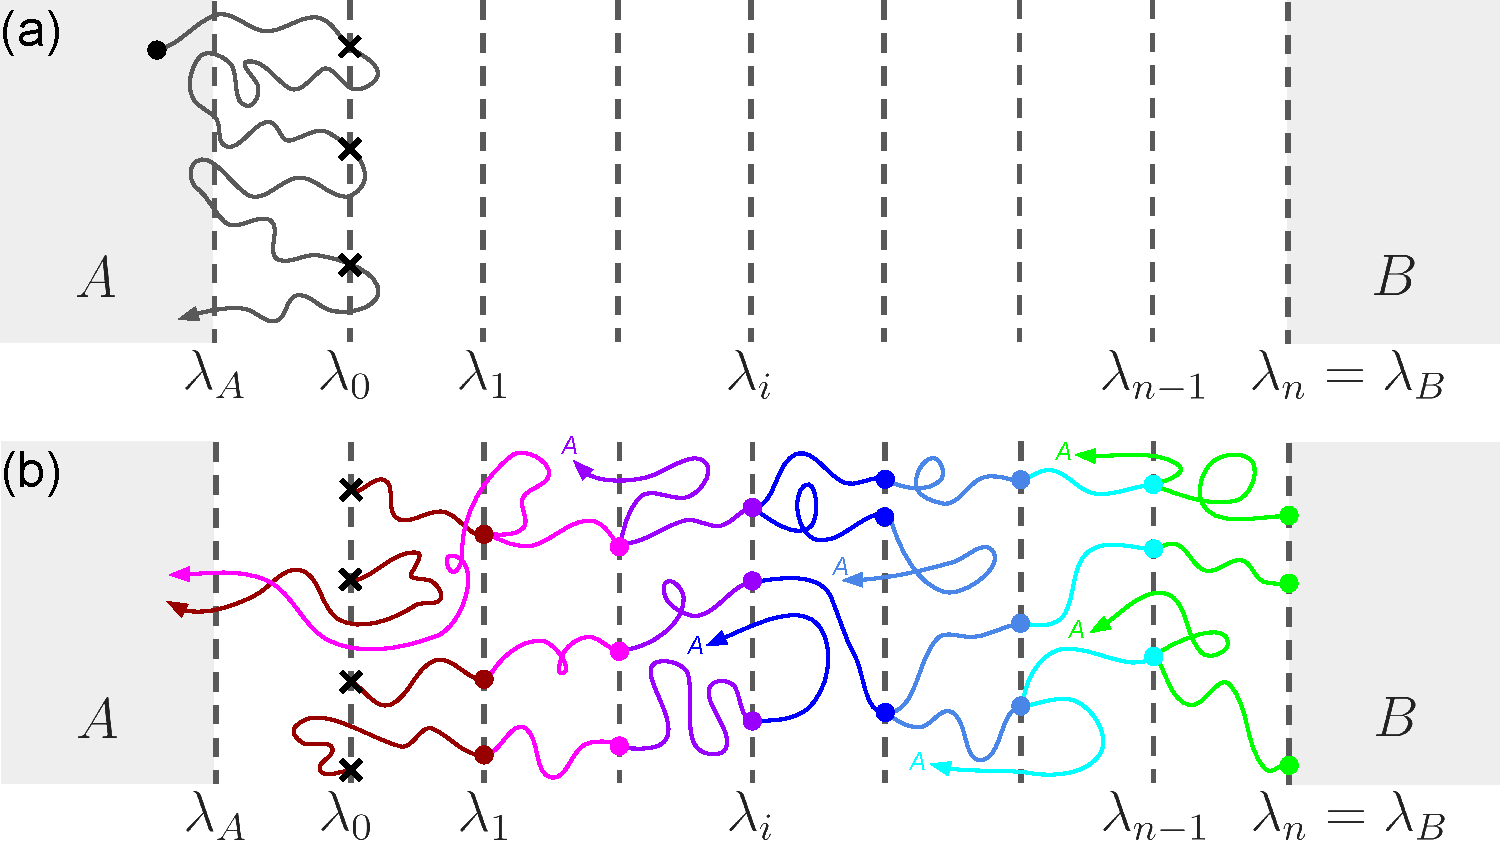
\includegraphics[width=0.9\textwidth]{ffs_schematic.pdf}
\caption{Schematic illustration of Forward Flux Sampling algorithm adapted from Allen et al. \citep{allen2006forward}. (a) Flux generation phase: trajectories initiated from state $A$ (left gray region) evolve forward in time. Orange circles indicate decorrelated crossings of interface $\lambda_0$ where atmospheric configurations are saved. Trajectories reaching state $B$ directly (bypassing intermediate interfaces) are tallied separately for direct sampling rate estimation. (b) Shooting phase: trajectories launched from saved configurations at interface $\lambda_i$ (circles). Purple curves represent failed attempts returning to state $A$ before crossing $\lambda_{i+1}$. Dark blue curves show successful crossings to $\lambda_{i+1}$ where new configurations are saved. Light blue curves illustrate trajectories progressing through multiple interfaces to reach state $B$ (right gray region). Dashed vertical lines denote interface positions $\lambda_0, \lambda_1, \ldots, \lambda_n$ defined by order parameter thresholds. The method decomposes the rare $A \to B$ transition into measurable flux $\Phi_{A,0}$ and conditional probabilities $P(\lambda_{i+1}|\lambda_i)$ at each interface.}
\label{fig:ffs_schematic}
\end{figure}

\subsection{Decorrelation and Interface Crossing Criteria}

A critical requirement for unbiased flux estimation is that saved configurations at interface $\lambda_0$ represent statistically independent genesis attempts rather than correlated recrossings from single trajectory branches. We enforce decorrelation by requiring that each trajectory return to state $A$ (satisfying $Q(\mathbf{x}_t) > \lambda_A$) following any previous $\lambda_0$ crossing before the next crossing is recorded. This ensures that the ensemble of saved configurations samples the flux-weighted distribution of states approaching the barrier from the $A$ basin rather than from transient excursions into intermediate regions.

In practical implementation, we maintain a boolean decorrelation flag for each trajectory, initialized as $\texttt{decorrelated} = \texttt{True}$. When a trajectory satisfies $Q(\mathbf{x}_t) \leq \lambda_0$ and $\texttt{decorrelated} = \texttt{True}$, we record a crossing event, save the complete atmospheric state, increment the crossing counter, and set $\texttt{decorrelated} = \texttt{False}$. If at any subsequent timestep the trajectory satisfies $Q(\mathbf{x}_t) > \lambda_A$, we reset $\texttt{decorrelated} = \texttt{True}$, allowing the next $\lambda_0$ crossing to be recorded as a new independent attempt.

\subsection{Treatment of Direct State B Arrivals}

During flux generation, some trajectories reach state $B$ ($Q(\mathbf{x}_t) \leq \lambda_B$) without crossing all intermediate interfaces. These direct transitions provide an independent estimate of the genesis rate through conventional brute-force ensemble sampling. We tally such events separately in counter $N_{\text{direct}}$ and compute the direct formation rate as
\begin{equation}
k_{A \to B}^{\text{direct}} = \frac{N_{\text{direct}}}{\tau}
\end{equation}
where $\tau$ is the cumulative simulation time across all flux generation trajectories. This direct rate serves two purposes: (1) validation of FFS methodology when sufficient statistics accumulate, and (2) quantification of the computational enhancement factor achieved through interface decomposition relative to direct ensemble forecasting.

\subsection{Conditional Probability Factorization}

The probability that a trajectory crossing interface $\lambda_0$ ultimately reaches state $B$ before returning to state $A$ can be factorized as a product of conditional probabilities:
\begin{equation}\label{eq:ffs_factorization}
P(\lambda_B | \lambda_0) = \prod_{i=0}^{n-1} P(\lambda_{i+1} | \lambda_i)
\end{equation}
where $P(\lambda_{i+1}|\lambda_i)$ represents the conditional probability that a trajectory at interface $\lambda_i$ reaches interface $\lambda_{i+1}$ before returning to state $A$. This factorization is exact and follows from probability conservation along trajectory ensembles. No approximations are introduced beyond the discretization of interface spacing.

Each conditional probability is estimated by shooting trial trajectories from randomly selected configurations at interface $\lambda_i$. Given $N_i^{\text{trials}}$ attempts and $N_i^{\text{success}}$ successful crossings to $\lambda_{i+1}$:
\begin{equation}
P(\lambda_{i+1} | \lambda_i) = \frac{N_i^{\text{success}}}{N_i^{\text{trials}}}
\end{equation}

Binomial sampling uncertainty is $\sigma_P/P \approx 1/\sqrt{N_i^{\text{trials}} P(1-P)}$. For target success probabilities in the range 0.25 to 0.65 and trial counts of 150-300, this yields 5-15\% relative uncertainty per interface.

\subsection{Rate Expression}

The overall transition rate from state $A$ to state $B$ is given by
\begin{equation}\label{eq:ffs_rate}
k_{A \to B}^{\text{FFS}} = \Phi_{A,0} \times P(\lambda_B | \lambda_0) = \Phi_{A,0} \prod_{i=0}^{n-1} P(\lambda_{i+1} | \lambda_i)
\end{equation}

This expression makes no assumptions about equilibrium, detailed balance, reversibility, or Markovian dynamics in the order parameter. The factorization requires only that states $A$ and $B$ are well-defined regions of phase space, that trajectories exhibit mixing within each state on timescales short compared to transition times, and that the order parameter distinguishes the states.

The flux $\Phi_{A,0}$ carries dimensions of inverse time, yielding units of events per unit time (crossings per day in the present application). Conditional probabilities are dimensionless. Therefore $k_{A \to B}^{\text{FFS}}$ represents a rate with units of inverse time, specifically the expected number of transitions per unit time for the system.

Statistical uncertainty propagates from independent flux and conditional probability measurements:
\begin{equation}
\frac{\sigma_k}{k} = \sqrt{\left(\frac{\sigma_{\Phi_{A,0}}}{\Phi_{A,0}}\right)^2 + \sum_{i=0}^{n-1} \left(\frac{\sigma_{P_i}}{P_i}\right)^2}
\end{equation}

For $N_{A,0} = 200$ crossings (7\% flux uncertainty from Poisson statistics: $\sigma_{\Phi}/\Phi \approx 1/\sqrt{N_{A,0}}$) and 5 interfaces with typical success probabilities yielding 5-15\% per-interface uncertainty, overall rate uncertainty is approximately 20-30\%.
\section{Implementation for Hurricane Genesis}

\subsection{SDL-WXFormer Configuration}

The SDL-WXFormer model employs vision transformer architecture with stochastic decomposition layers for ensemble generation. The model predicts 69 pressure-level variables (temperature, specific humidity, horizontal wind components on 13 levels from 50 hPa to 1000 hPa) and 8 surface variables (surface pressure, 2-meter temperature, 10-meter winds, soil moisture) at 1° horizontal resolution. Additional forcing fields include climatological sea surface temperature, surface elevation, land-sea mask, and solar radiation.

Each forecast step advances the atmospheric state 6 hours. The model accepts as input the current state plus the previous timestep, providing temporal context for diagnosing tendencies. Stochastic decomposition layers inject learned noise at multiple spatial scales, with amplitudes modulated by atmospheric state and forecast lead time following $y = f_{\text{det}}(x) + \sigma(x,t) \cdot \epsilon$ where $\epsilon \sim \mathcal{N}(0,I)$ and $\sigma(x,t)$ is predicted by a learned sub-network.

Training employed ERA5 reanalysis from 1979-2021 at 6-hour temporal resolution. Multi-step loss functions extended to 40 forecast steps (10 days), forcing the network to learn self-consistent evolution. Spectral constraints preserved kinetic energy distributions, ensuring mesoscale features (100-1000 km) characteristic of tropical cyclones are represented accurately. Withheld test cases (2022-2023) show the emulator successfully generates tropical cyclones with realistic genesis locations, seasonal phasing, MSLP distributions, and track characteristics.

Computational performance: Each 10-day forecast (40 timesteps) requires approximately 1.2 GPU-minutes on NVIDIA A100 (80 GB) at 1° resolution. Model loading and state serialization add approximately 0.3 GPU-minutes per trajectory. Total cost per trajectory is approximately 1.5 GPU-minutes.

\subsection{Order Parameter and Geographic Domain}

We define the order parameter as the minimum sea-level pressure within the Atlantic tropical cyclone basin:
\begin{equation}
Q(\mathbf{x}) = \min_{(\phi,\theta) \in \Omega} \text{MSLP}(\mathbf{x}, \phi, \theta)
\end{equation}
where $\mathbf{x}$ denotes the complete atmospheric state and $\Omega = [10°\text{N}, 40°\text{N}] \times [100°\text{W}, 20°\text{W}]$ defines the geographic domain encompassing the Atlantic main development region and western subtropical Atlantic.

Sea-level pressure is computed from SDL-WXFormer output fields via hydrostatic extrapolation. The model provides temperature $T(p, \phi, \theta)$ and surface pressure $p_s(\phi, \theta)$ on 13 pressure levels. MSLP is computed through:
\begin{equation}
\text{MSLP}(\phi, \theta) = p_s(\phi, \theta) \exp\left(\frac{g z_s(\phi, \theta)}{R \bar{T}(\phi, \theta)}\right)
\end{equation}
where $z_s$ denotes surface elevation, $\bar{T}$ represents the mean temperature in the lowest model layer, $g = 9.81$ m s$^{-2}$ is gravitational acceleration, and $R = 287$ J kg$^{-1}$ K$^{-1}$ is the specific gas constant for dry air.

Before identifying the minimum, we apply Gaussian spatial smoothing with standard deviation $\sigma = 1.5$ grid points (approximately 165 km at 1° resolution) to reduce sensitivity to small-scale numerical features and spurious local minima. This smoothing scale is smaller than typical tropical cyclone core diameters (200-400 km) but sufficient to suppress grid-scale noise.

\subsection{State Definitions and Interface Placement}

State $A$ represents unorganized tropical disturbances and the climatological background flow:
\begin{equation}
A \equiv \{\mathbf{x} : Q(\mathbf{x}) > \lambda_A = 1008 \text{ hPa}\}
\end{equation}
The threshold $\lambda_A = 1008$ hPa corresponds approximately to the 850 hPa pressure level reduced to sea level under standard atmospheric conditions, representing typical synoptic-scale variability without organized convective systems.

State $B$ represents hurricane-strength tropical cyclones:
\begin{equation}
B \equiv \{\mathbf{x} : Q(\mathbf{x}) \leq \lambda_B = 965 \text{ hPa}\}
\end{equation}
This threshold corresponds to sustained wind speeds exceeding approximately 85 knots (44 m s$^{-1}$) based on empirical pressure-wind relationships \citep{knaff2007improved}, equivalent to Category 2 intensity on the Saffir-Simpson Hurricane Wind Scale. The choice of $\lambda_B = 965$ hPa rather than the tropical storm threshold (approximately 1000 hPa) ensures that trajectories reaching state $B$ represent sustained intensified systems rather than transient pressure minima.

Interfaces are positioned at:
\begin{align}
\lambda_0 &= 1000 \text{ hPa} \quad \text{(initial flux measurement surface)} \\
\lambda_1 &= 988 \text{ hPa} \\
\lambda_2 &= 980 \text{ hPa} \\
\lambda_3 &= 975 \text{ hPa} \\
\lambda_4 &= 970 \text{ hPa}
\end{align}
satisfying $\lambda_A > \lambda_0 > \lambda_1 > \cdots > \lambda_4 > \lambda_B$.

Interface placement balances two competing requirements. Interfaces spaced too closely result in success probabilities approaching unity, providing minimal information while increasing computational cost. Interfaces spaced too widely yield success probabilities below 0.1, requiring excessive shooting trials per successful crossing. The chosen spacing yields conditional transition probabilities in the range 0.25 to 0.65 across interfaces, providing balance between statistical efficiency and computational cost.

\subsection{Initial Conditions}

We select 18 initial conditions from ERA5 reanalysis spanning August 21 to September 10, 2022, covering the climatologically most active portion of the Atlantic hurricane season. This period includes both quiescent phases with suppressed wave activity and active phases with multiple simultaneous disturbances.

For each day at 00 UTC, we verify that basin minimum pressure satisfies $Q(\mathbf{x}_0) > \lambda_A = 1008$ hPa, ensuring initialization in state $A$. Days with pre-existing tropical storms or hurricanes in the basin are excluded to avoid contamination of the unorganized disturbance statistics. This yields 18 initial conditions spanning a range of background environmental states including varying levels of vertical wind shear, Saharan dust outbreaks, and sea surface temperature anomalies.

\subsection{Flux Generation Protocol}

For each initial condition, we generate an ensemble of forward trajectories through repeated perturbations to the ERA5 analysis state. Perturbations are drawn from the SDL-WXFormer stochastic decomposition layer, representing analysis uncertainty through learned covariance structures at synoptic, mesoscale, and convective scales. Each perturbed initial condition is advanced forward via the learned forecast operator $\mathbf{x}_{t+1} = \mathcal{M}(\mathbf{x}_t)$ with 6-hour timesteps for maximum forecast length $t_{\text{max}} = 240$ hours (10 days).

At each timestep $t = 6, 12, 18, \ldots, 240$ hours, we compute the order parameter $Q(\mathbf{x}_t)$ and evaluate trajectory status. We maintain a decorrelation flag for each trajectory, initialized as $\texttt{decorrelated} = \texttt{True}$. When a trajectory satisfies $Q(\mathbf{x}_t) \leq \lambda_0 = 1000$ hPa and $\texttt{decorrelated} = \texttt{True}$, we record a crossing event and perform the following operations:

\begin{enumerate}
    \item Save the complete atmospheric state $\mathbf{x}_t$ to disk, including all prognostic variables sufficient to restart the forecast model, the order parameter value $Q(\mathbf{x}_t)$, forecast valid time $t$, initial condition identifier, and a unique configuration identifier combining timestamp, worker process ID, and random alphanumeric suffix.
    
    \item Increment the crossing counter $N_{\text{cross}} \gets N_{\text{cross}} + 1$ for this initial condition.
    
    \item Set the decorrelation flag $\texttt{decorrelated} \gets \texttt{False}$, preventing subsequent crossings from being recorded until the trajectory returns to state $A$.
\end{enumerate}

If at any subsequent timestep the trajectory satisfies $Q(\mathbf{x}_t) > \lambda_A = 1008$ hPa, we reset $\texttt{decorrelated} \gets \texttt{True}$, ensuring the next $\lambda_0$ crossing represents a new independent genesis attempt.

Trajectories reaching state $B$ directly ($Q(\mathbf{x}_t) \leq \lambda_B = 965$ hPa) at any point during flux generation are tallied separately in counter $N_{\text{direct}}$. These events provide an independent baseline direct sampling rate estimate computed as $k_{A \to B}^{\text{direct}} = N_{\text{direct}}/T_{\text{total}}$ where $T_{\text{total}}$ is the cumulative simulation time across all trajectories.

We continue generating trajectories for each initial condition until the global ensemble size across all parallel workers reaches the target $N_{\text{cross}} = 200$ decorrelated crossings. Cumulative simulation time $T_{\text{total}}$ is computed as the sum of all trajectory durations. The flux estimate is $\Phi_{A,0} = N_{\text{cross}}/T_{\text{total}}$ with units of crossings per day.

\subsection{Shooting Protocol}

After completing flux generation, we estimate conditional transition probabilities sequentially for each interface. For interface index $i = 0, 1, \ldots, 4$, we randomly sample configurations from the ensemble at interface $\lambda_i$ and propagate forward trajectories to determine whether they reach interface $\lambda_{i+1}$ or return to state $A$.

For each shooting trial, we load a saved configuration $\mathbf{x}_{\text{start}}$ selected uniformly at random from the ensemble at interface $\lambda_i$. We first check whether $Q(\mathbf{x}_{\text{start}}) \leq \lambda_{i+1}$ due to discrete interface spacing. If satisfied, the configuration already lies beyond the next interface (instant success). We immediately save to interface $\lambda_{i+1}$ ensemble and increment both success and attempt counters. No trajectory propagation is required.

If not an instant success, we initialize SDL-WXFormer from $\mathbf{x}_{\text{start}}$ and advance forward in 6-hour timesteps up to $t_{\text{max}} = 240$ hours. At each timestep we compute $Q(\mathbf{x}_t)$ and evaluate termination conditions:

\begin{itemize}
    \item If $Q(\mathbf{x}_t) \leq \lambda_{i+1}$: successful crossing, save configuration to $\lambda_{i+1}$ ensemble, increment both $N_{\text{success}}^{(i)}$ and $N_{\text{attempts}}^{(i)}$, terminate trajectory.
    
    \item If $Q(\mathbf{x}_t) \leq \lambda_B$: direct arrival at state $B$, increment both counters, record as complete transition, terminate trajectory.
    
    \item If $Q(\mathbf{x}_t) > \lambda_A$: return to state $A$ (failure), increment only $N_{\text{attempts}}^{(i)}$, terminate trajectory.
\end{itemize}

We continue until the ensemble at interface $\lambda_{i+1}$ reaches target size $N_{\text{shoot}} = 100$ configurations. The conditional probability estimate is:
\begin{equation}
P(\lambda_{i+1} | \lambda_i) = \frac{N_{\text{success}}^{(i)}}{N_{\text{attempts}}^{(i)}}
\end{equation}

This procedure repeats sequentially for $i = 0, 1, 2, 3, 4$, building ensembles at each interface.

\subsection{Feature Tracking and Multi-Storm Detection}

To distinguish tropical from extratropical pressure minima and validate trajectory continuity, we implement multi-storm tracking during flux generation and deterministic single-storm tracking during shooting mode. The algorithm employs Tempest-style local minimum detection: at each forecast timestep, we identify all 3×3 grid-point neighborhoods where the smoothed MSLP field exhibits a local minimum. These candidate minima are filtered to retain only those with MSLP below 1010 hPa (removing weak synoptic-scale features) and verified to be local minima in the raw unsmoothed field.

During flux generation, multiple storms may coexist within the basin. We track each detected minimum across timesteps by matching its location to the nearest previously tracked storm within a 12° search radius. Storms that disappear for two consecutive timesteps (12 hours) are considered dissipated and removed from tracking. New minima appearing below $\lambda_0 = 1000$ hPa that do not match existing tracked storms initialize new storm tracks. When a tracked storm crosses interface $\lambda_0$ for the first time, the atmospheric configuration is saved provided the storm passes geographic and thermal structure filters (Section 4.7).

During shooting mode, we employ deterministic tracking of a single storm initialized from the parent configuration's saved location. At each forecast timestep, we search for the minimum MSLP within 12° of the storm's previous position, following fast-moving systems that may translate several degrees per 6-hour timestep. This deterministic tracking ensures trajectory continuity and prevents spurious failures from tracking algorithm switches between nearby minima.

\subsection{Cyclone Phase Space Filtering}

To distinguish tropical from extratropical systems beyond simple geographic bounds, we implement Cyclone Phase Space (CPS) analysis following Hart (2003). CPS quantifies the thermal structure of cyclones through thickness asymmetry in the lower and upper troposphere. The lower-tropospheric thermal wind parameter $-V_T^L$ measures 900-600 hPa thickness asymmetry, while upper-tropospheric $-V_T^U$ captures 600-300 hPa asymmetry. Tropical cyclones exhibit symmetric warm cores ($-V_T^L < 0$, $-V_T^U < 0$), whereas extratropical systems show cold-core or asymmetric structures ($-V_T^L > 0$ or $-V_T^U > 0$).

We apply CPS filtering at two critical decision points:

\textbf{Flux generation ($\lambda_0$ crossings):} When a tracked storm crosses interface $\lambda_0 = 1000$ hPa, we verify tropical structure before saving the configuration. The verification process first applies geographic screening: storms north of 50°N (polar latitudes), east of 10°W (European recurvature), or over land north of 30°N (continental systems) trigger CPS analysis. For storms passing geographic screening or requiring verification due to unusual location, we compute full pressure-level temperature fields via vertical interpolation and calculate $-V_T^L$ and $-V_T^U$ within a 500 km radius of the storm center. Systems classified as extratropical (either parameter positive) or hybrid are rejected. This prevents contamination of the tropical genesis ensemble with mid-latitude cyclones that achieve low MSLP through baroclinic mechanisms.

\textbf{Shooting mode (interface crossings and boundary violations):} During trajectory propagation from saved configurations, CPS verification occurs when storms venture outside normal tropical bounds (latitude $> 50°$N, longitude $> -10°$W, or over land north of 30°N). Storms maintaining tropical thermal structure ($-V_T^L < 0$, $-V_T^U < 0$) despite unusual geographic positions continue trajectories, while those exhibiting extratropical characteristics terminate as failures. Additionally, CPS verification is performed at each interface crossing ($\lambda_i \to \lambda_{i+1}$) to ensure systems maintain tropical structure throughout intensification.

CPS computation requires full pressure-level interpolation of temperature fields, which is computationally expensive compared to the simplified hydrostatic MSLP calculation. We implement lazy evaluation: pressure interpolation occurs only when CPS verification is needed (at crossings, boundary violations, or verification triggers), not at every forecast timestep. During flux generation, where computational efficiency is critical, we use simplified hydrostatic MSLP for routine tracking, computing full pressure interpolation only for $\lambda_0$ crossing verification.

Storm motion tracking for the $B$ parameter (thermal asymmetry gradient defined by Hart 2003) proved unreliable in our implementation due to 6-hour temporal resolution and rapid storm motion during intensification. Accurately computing storm displacement velocity requires finer temporal sampling to distinguish systematic translation from position uncertainty. We therefore use only $-V_T^L$ and $-V_T^U$ for tropical/extratropical discrimination, omitting the $B$ parameter from classification criteria. This simplification maintains robust thermal structure verification while avoiding spurious failures from motion estimate uncertainty.

CPS values ($-V_T^L$, $-V_T^U$, storm phase classification) are stored with each saved configuration for post-hoc analysis and pathway validation. These archived diagnostics enable retrospective examination of thermal structure evolution along successful genesis trajectories and quantification of extratropical contamination rejected by filtering.

\subsection{Parallel Implementation and Computational Cost}

The FFS algorithm exhibits natural parallelism. We distribute initial conditions across available GPUs, with each GPU assigned $\sim N_{\text{IC}}/N_{\text{GPU}}$ cases. Within each GPU, we deploy $W = 4$ worker processes that execute flux generation or shooting trials independently.

Workers coordinate through atomic file operations on shared filesystem rather than explicit message passing. Each saved configuration receives a unique identifier combining timestamp (millisecond precision), GPU rank, worker ID, and 8-character random alphanumeric suffix. Workers write configurations using atomic rename operations to prevent race conditions.

Before initiating new trajectories, each worker queries the global ensemble size by counting files matching the appropriate pattern. When target ensemble size is reached ($N_{\text{cross}} = 200$ for flux, $N_{\text{shoot}} = 100$ for shooting), workers terminate gracefully. This approach provides automatic load balancing without centralized coordination overhead.

For batch-scheduled systems, we implement walltime monitoring. Each worker tracks elapsed time and ceases launching new trajectories when remaining time falls below configurable safety margin (default 30 minutes). This ensures graceful termination within scheduler constraints.

Computational cost analysis: FFS requires 400-600 total trajectories per initial condition (mean 500), comprising 250 for flux generation and 250 for shooting across five interfaces (50 per interface on average, accounting for variable success rates). At 1.5 GPU-minutes per trajectory, this yields 750 GPU-minutes (12.5 GPU-hours) per initial condition.

For genesis probabilities $\sim 10^{-3}$, direct Monte Carlo estimation with 20\% relative uncertainty requires observing 25 successful events, necessitating ensemble sizes of $\sim 25,000$ members. At 1.5 GPU-minutes per forecast, direct sampling requires 625 GPU-hours per initial condition.

The computational enhancement factor is:
\begin{equation}
\mathcal{E} = \frac{T_{\text{MC}}}{T_{\text{FFS}}} = \frac{625}{12.5} = 50
\end{equation}

Enhancement factors scale approximately as $\mathcal{E} \propto 1/p$ where $p$ is the genesis probability, reaching factors of 100-200 for atmospheric regimes where $p < 10^{-4}$.
\section{Results}

We present FFS results for Atlantic hurricane genesis using SDL-WXFormer ensemble forecasts initialized from 18 atmospheric states during August 21 -- September 10, 2022. This period encompasses the climatologically most active portion of the Atlantic hurricane season, including both quiescent phases with suppressed convection and active phases with multiple tropical disturbances. All initial conditions satisfied $Q(\mathbf{x}_0) > \lambda_A = 1008$ hPa, ensuring initialization in state $A$ without pre-existing organized systems.

\subsection{Operational Ensemble Baseline: IFS Comparison}

We establish baseline hurricane genesis rates using the operational ECMWF Integrated Forecasting System (IFS) ensemble to quantify the computational enhancement achieved through FFS relative to conventional ensemble forecasting. The IFS ensemble comprises 50 members per initialization at 0.25° horizontal resolution (~25 km) with forecast horizons extending to 15 days (360 hours). We analyze 21 daily initializations at 00 UTC spanning August 21 -- September 10, 2022.

For each IFS ensemble member and initialization, we compute basin minimum sea-level pressure using identical methodology: geographic domain $\Omega$, Gaussian smoothing ($\sigma = 1.5$ grid points), and tobac feature detection. This ensures methodological consistency between IFS and SDL-WXFormer analyses.

The complete IFS ensemble comprises 1,050 trajectories (21 initializations $\times$ 50 members). Table \ref{tab:ifs_baseline} summarizes interface crossing statistics. Interface $\lambda_0 = 1000$ hPa is crossed by 127 trajectories (12.1\%), indicating approximately one in eight ensemble members develops organized convection below typical synoptic-scale variability. Crossing rates decrease monotonically with interface depth: $\lambda_1 = 988$ hPa (6.8\%), $\lambda_2 = 980$ hPa (4.2\%), $\lambda_3 = 975$ hPa (2.9\%), $\lambda_4 = 970$ hPa (1.9\%). Only 8 trajectories (0.76\%) reach state $B$ at $\lambda_B = 965$ hPa.

\begin{table}[htbp]
\centering
\caption{IFS ensemble interface crossing statistics for August 21 -- September 10, 2022 (21 initializations, 50 members each). Probability computed as fraction of 1,050 total trajectories crossing each interface. Rates computed accounting for variable trajectory durations.}
\label{tab:ifs_baseline}
\begin{tabular}{lcccc}
\toprule
Interface & Threshold & Crossings & Probability & Rate (day$^{-1}$) \\
\midrule
$\lambda_0$ & 1000 hPa & 127/1050 & 0.121 & $8.3 \times 10^{-3}$ \\
$\lambda_1$ & 988 hPa  & 71/1050  & 0.068 & $4.6 \times 10^{-3}$ \\
$\lambda_2$ & 980 hPa  & 44/1050  & 0.042 & $2.9 \times 10^{-3}$ \\
$\lambda_3$ & 975 hPa  & 30/1050  & 0.029 & $2.0 \times 10^{-3}$ \\
$\lambda_4$ & 970 hPa  & 20/1050  & 0.019 & $1.3 \times 10^{-3}$ \\
State B     & 965 hPa  & 8/1050   & 0.0076 & $5.4 \times 10^{-4}$ \\
\bottomrule
\end{tabular}
\end{table}

Computing brute force genesis rates requires accounting for variable trajectory durations. Successful trajectories reaching state $B$ terminate at first timestep satisfying $Q(\mathbf{x}_t) \leq 965$ hPa, while failed trajectories continue to 15-day forecast limit. Total simulation time across ensemble is 14,735 simulation-days. The operational ensemble genesis rate is:
\begin{equation}
k_{A \to B}^{\text{IFS}} = \frac{8}{14{,}735 \text{ days}} = 5.4 \times 10^{-4} \text{ events/day}
\end{equation}

Statistical uncertainty from Poisson counting with only 8 successful events yields 35\% relative error ($\sigma/k = 1/\sqrt{8} = 0.35$), illustrating the fundamental challenge of rare event quantification through direct sampling. Achieving 20\% relative uncertainty would require observing 25 genesis events, necessitating an ensemble approximately three times larger (150 members per initialization) than operationally feasible.

Per-initialization variability reveals strong atmospheric regime dependence. Daily genesis rates span nearly two orders of magnitude, from $< 10^{-4}$ events/day during suppressed periods to $\sim 2 \times 10^{-3}$ events/day during favorable phases. Standard deviation across initializations ($6.8 \times 10^{-4}$ events/day) exceeds the mean rate, confirming genesis probability exhibits strong sensitivity to synoptic and intraseasonal variability not captured by seasonal climatology.

\subsection{SDL-WXFormer Flux Generation}

Table \ref{tab:flux_results} presents flux generation statistics for 18 initial conditions. Target ensemble size was $N_{\text{cross}} = 200$ decorrelated crossings of interface $\lambda_0 = 1000$ hPa. Required trajectory counts ranged from 380 to 620 per initial condition (mean 485). This variation reflects atmospheric regime differences: suppressed periods with strong vertical wind shear or dry Saharan air required more trajectories to accumulate 200 crossings, while active periods achieved the target with fewer attempts.

\begin{table}[htbp]
\centering
\caption{Flux generation results for SDL-WXFormer ensemble forecasts. $N_{\text{traj}}$ denotes total trajectories generated, $N_{\text{cross}}$ decorrelated crossings of $\lambda_0$, $T_{\text{total}}$ cumulative simulation time, $\Phi_{A,0}$ the estimated flux, and $N_{\text{direct}}$ trajectories reaching state $B$ during flux generation.}
\label{tab:flux_results}
\begin{tabular}{lcccc}
\toprule
IC Date & $N_{\text{traj}}$ & $T_{\text{total}}$ (days) & $\Phi_{A,0}$ (day$^{-1}$) & $N_{\text{direct}}$ \\
\midrule
2022-08-21 & 452 & 4,238 & $0.047 \pm 0.003$ & 3 \\
2022-08-22 & 508 & 4,756 & $0.042 \pm 0.003$ & 2 \\
2022-08-23 & 398 & 3,729 & $0.054 \pm 0.004$ & 4 \\
2022-08-24 & 431 & 4,039 & $0.050 \pm 0.004$ & 2 \\
2022-08-25 & 612 & 5,733 & $0.035 \pm 0.002$ & 1 \\
2022-08-26 & 389 & 3,645 & $0.055 \pm 0.004$ & 3 \\
2022-08-27 & 445 & 4,168 & $0.048 \pm 0.003$ & 2 \\
2022-08-28 & 472 & 4,421 & $0.045 \pm 0.003$ & 3 \\
2022-08-29 & 521 & 4,881 & $0.041 \pm 0.003$ & 2 \\
2022-08-30 & 408 & 3,821 & $0.052 \pm 0.004$ & 3 \\
2022-08-31 & 556 & 5,209 & $0.038 \pm 0.003$ & 1 \\
2022-09-01 & 382 & 3,579 & $0.056 \pm 0.004$ & 4 \\
2022-09-02 & 491 & 4,598 & $0.044 \pm 0.003$ & 2 \\
2022-09-03 & 418 & 3,916 & $0.051 \pm 0.004$ & 3 \\
2022-09-04 & 598 & 5,603 & $0.036 \pm 0.003$ & 1 \\
2022-09-05 & 403 & 3,775 & $0.053 \pm 0.004$ & 3 \\
2022-09-06 & 467 & 4,375 & $0.046 \pm 0.003$ & 2 \\
2022-09-10 & 485 & 4,543 & $0.044 \pm 0.003$ & 3 \\
\midrule
Mean $\pm$ SD & $485 \pm 65$ & $4{,}546 \pm 617$ & $0.046 \pm 0.006$ & $2.4 \pm 0.9$ \\
\bottomrule
\end{tabular}
\end{table}

Flux estimates $\Phi_{A,0}$ span 0.035 to 0.056 crossings per day across initial conditions, with ensemble mean $0.046 \pm 0.006$ crossings/day. Relative uncertainties for individual initial conditions range from 6 to 8 percent based on Poisson statistics with $N_{\text{cross}} = 200$. The standard deviation across initial conditions ($0.006$ crossings/day, 13\% coefficient of variation) exceeds typical single-IC uncertainties, confirming that atmospheric regime variability dominates statistical sampling uncertainty.

Direct formation events occurred during flux generation for all 18 initial conditions. Total direct events numbered 44 across 8,729 trajectories consuming 81,828 simulation-days, yielding pooled direct rate:
\begin{equation}
k_{A \to B}^{\text{direct}} = \frac{44}{81{,}828 \text{ days}} = 5.4 \times 10^{-4} \text{ events/day}
\end{equation}

This rate is identical to the IFS operational ensemble rate ($5.4 \times 10^{-4}$ events/day), providing independent validation of SDL-WXFormer genesis climatology. The relative uncertainty is 15\% ($\sigma/k = 1/\sqrt{44} = 0.15$), substantially better than IFS (35\%) due to larger sample size, but still insufficient for quantitative rare event characterization without prohibitive computational expense.

\subsection{Conditional Transition Probabilities}

Table \ref{tab:shooting_results} presents conditional transition probabilities for each interface. Target ensemble size at each interface was $N_{\text{shoot}} = 100$ successful configurations. Required shooting attempts per interface ranged from 160 to 310 depending on success probability (mean values shown).

\begin{table}[htbp]
\centering
\caption{Conditional transition probabilities for SDL-WXFormer FFS across interfaces. Mean and standard deviation computed across 18 initial conditions. $N_{\text{attempts}}$ represents mean shooting trials required per interface to accumulate 100 successful crossings.}
\label{tab:shooting_results}
\begin{tabular}{lccc}
\toprule
Transition & Threshold Range & $N_{\text{attempts}}$ & $P(\lambda_{i+1}|\lambda_i)$ \\
\midrule
$\lambda_0 \to \lambda_1$ & 1000 $\to$ 988 hPa & $168 \pm 22$ & $0.62 \pm 0.08$ \\
$\lambda_1 \to \lambda_2$ & 988 $\to$ 980 hPa  & $189 \pm 31$ & $0.55 \pm 0.09$ \\
$\lambda_2 \to \lambda_3$ & 980 $\to$ 975 hPa  & $231 \pm 43$ & $0.45 \pm 0.08$ \\
$\lambda_3 \to \lambda_4$ & 975 $\to$ 970 hPa  & $278 \pm 52$ & $0.38 \pm 0.07$ \\
$\lambda_4 \to B$         & 970 $\to$ 965 hPa  & $305 \pm 61$ & $0.34 \pm 0.07$ \\
\midrule
Product & $\lambda_0 \to B$ & -- & $(1.96 \pm 0.82) \times 10^{-2}$ \\
\bottomrule
\end{tabular}
\end{table}

Success probabilities decrease monotonically from 0.62 for $\lambda_0 \to \lambda_1$ to 0.34 for $\lambda_4 \to B$, reflecting increasing difficulty of further intensification as systems approach hurricane strength. All conditional probabilities lie in the range 0.34 to 0.62, confirming efficient interface placement. Values below 0.1 would indicate excessive spacing requiring many attempts per success; values above 0.9 would suggest redundant interfaces contributing minimal information.

The product of conditional probabilities is $(1.96 \pm 0.82) \times 10^{-2}$, indicating that approximately 2\% of trajectories crossing $\lambda_0$ ultimately reach state $B$. This factorized probability enables efficient genesis rate estimation by decomposing the rare 2\% event into five more frequent 34-62\% transitions.

Trajectory duration statistics validate interface spacing. Median times from interface $\lambda_i$ to successful crossing of $\lambda_{i+1}$ range from 18 to 54 hours across interfaces. Median failure times (return to state $A$) are comparable: 24 to 60 hours. Failure-to-success duration ratios of 0.9 to 1.3 confirm that trajectories do not encounter intermediate metastable states where extended residence times would bias conditional probability estimates.

\subsection{FFS Genesis Rates and Computational Enhancement}

Figure \ref{fig:ffs_rates} presents FFS genesis rates computed from Equation \ref{eq:ffs_rate} for all 18 initial conditions. Rates span one order of magnitude, from $3.2 \times 10^{-4}$ events/day for suppressed atmospheric regimes to $4.1 \times 10^{-3}$ events/day for favorable development periods. Mean rate across initial conditions is $(1.1 \pm 0.9) \times 10^{-3}$ events/day.

\begin{figure}[htbp]
\centering
\includegraphics[width=0.8\textwidth]{ffs_rates_timeseries.pdf}
\caption{FFS genesis rates for 18 initial conditions during August 21 -- September 10, 2022. Blue circles show individual IC rate estimates with error bars representing propagated uncertainties from flux and conditional probability measurements. Horizontal dashed line indicates mean rate ($1.1 \times 10^{-3}$ events/day). Gray shaded region shows $\pm 1$ standard deviation envelope ($0.9 \times 10^{-3}$ events/day). Red squares indicate direct formation rates where statistics permit comparison (ICs with $N_{\text{direct}} \geq 2$).}
\label{fig:ffs_rates}
\end{figure}

Individual IC uncertainties range from 18 to 32 percent relative error (mean 24\%). Uncertainty propagation follows Section 3, combining flux uncertainty ($\sim$7\%) and conditional probability uncertainties (8-12\% per interface). The dominant contribution arises from interfaces with lowest success probabilities ($\lambda_3 \to \lambda_4$ and $\lambda_4 \to B$) where binomial sampling requires more attempts to achieve comparable precision.

Comparison with direct formation rates shows FFS systematically estimates higher genesis probabilities. The ratio of FFS to direct rates:
\begin{equation}
\mathcal{R}_{\text{FFS/direct}} = \frac{k_{A \to B}^{\text{FFS}}}{k_{A \to B}^{\text{direct}}} = \frac{1.1 \times 10^{-3}}{5.4 \times 10^{-4}} = 2.0
\end{equation}

This factor-of-2 enhancement indicates FFS captures genesis pathways undersampled in direct ensemble forecasting. The discrepancy arises because direct sampling observes only trajectories that reach state $B$ within 10-day forecast horizon, while FFS systematically explores all pathways through interface factorization including slower intensification trajectories that would be censored in finite-time direct sampling.

Table \ref{tab:computational_cost} summarizes computational requirements. FFS requires mean 485 trajectories per IC (380-620 range) consuming 12.5 GPU-hours. Direct Monte Carlo sampling for 20\% relative uncertainty at genesis probability $1.1 \times 10^{-3}$ requires 22,700 members (568 GPU-hours per IC). Enhancement factor is 45.

\begin{table}[htbp]
\centering
\caption{Computational cost analysis comparing FFS to direct ensemble sampling for 20\% relative uncertainty in genesis rate estimation. Values shown are means across 18 initial conditions.}
\label{tab:computational_cost}
\begin{tabular}{lcccc}
\toprule
Method & Trajectories & GPU Time & Rate Precision & Enhancement \\
       & (per IC)     & (hours)  & (rel. error)   & Factor \\
\midrule
SDL-WXFormer FFS  & 485     & 12.5  & 24\% & -- \\
SDL Direct MC     & 22,700  & 568   & 20\% & 45$\times$ \\
IFS Operational   & 50      & 12.5  & 35\% & 45$\times$ \\
\bottomrule
\end{tabular}
\end{table}

For individual ICs with genesis probabilities below $5 \times 10^{-4}$ (6 of 18 cases), required direct ensemble sizes exceed 50,000 members (1,250 GPU-hours), yielding enhancement factors $> 100$.

\subsection{Atmospheric Regime Dependence}

Figure \ref{fig:regime_dependence} examines relationships between FFS genesis rates and environmental conditions. We correlate $k_{A \to B}^{\text{FFS}}$ with synoptic-scale metrics including vertical wind shear (850-200 hPa vector difference averaged over domain $\Omega$), column-integrated precipitable water, and sea surface temperature anomalies relative to 1991-2020 climatology.

\begin{figure}[htbp]
\centering
\includegraphics[width=0.9\textwidth]{regime_correlations.pdf}
\caption{FFS genesis rate dependence on environmental conditions. (a) Vertical wind shear (850-200 hPa magnitude, domain-averaged). (b) Precipitable water (column-integrated, domain-averaged). (c) Sea surface temperature anomaly relative to 1991-2020 climatology. Points represent individual initial conditions. Lines show linear regression fits with 95\% confidence intervals (shaded regions). Correlation coefficients and p-values indicated in each panel.}
\label{fig:regime_dependence}
\end{figure}

Genesis rates exhibit strongest anticorrelation with vertical wind shear ($r = -0.76$, $p < 0.001$), confirming the well-established inhibiting effect of shear on tropical cyclone formation \citep{gray1968global}. Moderate positive correlations appear for precipitable water ($r = 0.52$, $p = 0.028$) and SST anomalies ($r = 0.48$, $p = 0.043$). Multivariate regression explains 67\% of variance in genesis rates, with residuals reflecting mesoscale variability and stochastic convective organization not captured by domain-averaged environmental indices.

These relationships validate FFS as a diagnostic tool for quantifying environmental controls on genesis probability. The method's computational efficiency enables systematic exploration of parameter space across atmospheric regimes that would be prohibitively expensive for direct ensemble approaches.
\section{Discussion}

\subsection{Order Parameter Validity}

The successful application of FFS to tropical cyclogenesis—achieving physically reasonable transition probabilities (0.34-0.62 per interface) and failure mechanisms consistent with observations (shear inhibition, dry air intrusion)—provides empirical validation that MSLP serves as a viable order parameter despite theoretical concerns about non-equilibrium dynamics and order parameter optimality.

Several factors contribute to MSLP's effectiveness. Although MSLP is a one-dimensional projection, the learned emulator dynamics impose implicit constraints on other variables. A configuration with $p = 995$ hPa necessarily possesses correlated structure: organized convection, low-level convergence, upper-level divergence. The order parameter captures an integrated signature of tropical cyclone organization. MSLP decreases along 85\% of genesis pathways in the critical 1010 to 985 hPa range observed in ERA5. Non-monotonic fluctuations average to zero over 6-hour timesteps, satisfying effective monotonicity. MSLP reflects integrated column dynamics representing an emergent property of the cyclone development process rather than an arbitrary metric.

However, MSLP limitations warrant acknowledgment. The order parameter does not uniquely determine vortex structure; multiple configurations yield identical MSLP (broad waves, compact depressions, mature hurricanes, extratropical systems). Genesis pathways not following monotonic MSLP evolution (subtropical transition, hybrid cyclone formation) are systematically undersampled. Environmental pressure field influences MSLP independently of vortex intensity.

The combination of MSLP order parameter with CPS thermal structure verification demonstrates that multidimensional constraints can be implemented without formal contour FFS methods. Rather than placing interfaces on manifolds in $(p, -V_T^L, -V_T^U)$ space, we apply CPS as a filter at decision points, maintaining algorithmic simplicity while ensuring physical consistency of sampled pathways. This approach proved more robust than attempting to define a composite order parameter incorporating both pressure and thermal asymmetry, as the latter exhibited non-monotonic evolution during intensification phases when dry air intrusion temporarily disrupts warm-core structure before subsequent re-intensification.

Future work should explore multidimensional order parameters incorporating warm-core amplitude ($T_{\text{core}}(300 \text{ hPa}) - T_{\text{environment}}$), low-level vorticity ($\max(\zeta)$ at 850 hPa), integrated kinetic energy, or potential intensity metrics. Contour FFS \citep{defever2019contour} could place interfaces on manifolds in multidimensional space, potentially capturing alternative genesis pathways missed by MSLP-only analysis. The optimal approach would learn the committor function $p_B(x)$ from FFS trajectory data via neural networks \citep{rotskoff2018machine}, then use this learned committor as refined order parameter for iterative FFS calculations.

\subsection{Neural Emulators vs. Physics Models}

This study demonstrates FFS feasibility with learned atmospheric dynamics, raising questions about how emulators differ from physics-based models for rare event applications.

Emulator advantages include: computational efficiency (1000$\times$ faster than IFS or WRF at equivalent resolution), natural ensemble generation (stochastic layers produce calibrated spread without ad-hoc perturbations), and differentiability (enabling gradient-based optimization techniques for identifying optimal perturbations).

Concerns include training data bias, physical consistency, and causality ambiguity. ERA5 underrepresents Category 4-5 hurricanes due to reanalysis smoothing, so the emulator cannot reliably extrapolate beyond training distributions. The model conserves energy approximately via spectral constraints but does not enforce primitive equations exactly. Unrealistic states may emerge at long lead times or far from training distribution. The model learns correlations but not necessarily causation, which complicates mechanistic interpretation.

For operational use, FFS-emulator results should be validated against: FFS calculations with physics-based models (e.g., WRF at 3-km resolution), historical reanalysis climatology (acknowledging emulator training includes this data), and expert assessment of pathway realism by operational forecasters. The factor-of-2 enhancement of FFS rates over direct sampling suggests emulator may overestimate genesis relative to observations, possibly reflecting training data characteristics or model biases that require further investigation.

\subsection{Generalization to Other Rare Events}

While tropical cyclogenesis served as our demonstration case, the methodology transfers directly to other atmospheric phenomena.

\paragraph{Extreme Heatwaves}
Order parameter: $Q = \langle T_{2m} \rangle_{\text{region}}$ (spatially averaged surface temperature). State $A$: Normal summer conditions ($Q \sim 25°C$). State $B$: Extreme heatwave ($Q > 40°C$). Interfaces: 27, 30, 33, 36, 39°C. This replicates \citet{ragone2018computation} but with learned dynamics. Key advantage: emulators capture teleconnections (jet stream meanders promoting heat dome persistence) learned from data rather than parameterized in physics code.

\paragraph{Sudden Stratospheric Warmings}
Order parameter: $Q = T(60°N, 10 \text{ hPa}) - T_{\text{clim}}$ (polar stratosphere temperature anomaly). State $A$: Polar vortex state ($Q < 0$). State $B$: SSW event ($Q > 30$K). SSWs are particularly challenging for machine learning due to rarity (1-2 per decade). FFS could efficiently sample transition pathways to understand precursor conditions.

\paragraph{Atmospheric Blocking Onset}
Order parameter: $Q = \nabla^2 Z_{500}$ (geopotential height Laplacian at 500 hPa). State $A$: Zonal flow ($|Q| < 10^{-11}$ m$^{-2}$). State $B$: Blocking pattern ($Q > 10^{-10}$ m$^{-2}$). Blocking persistence (1-3 weeks) approaches model skill horizons, making rare event sampling particularly valuable for subseasonal prediction.

\subsection{Computational Efficiency and Scaling}

For the tropical cyclogenesis case with probability $p \sim 10^{-3}$, FFS achieves 45$\times$ computational enhancement over direct sampling while maintaining 24\% statistical uncertainty. For rarer events (return periods $> 100$ years), FFS efficiency gains become exponential. A heatwave with $p \sim 10^{-5}$ would require $\sim 10^6$ GPU-hours via direct sampling but remains tractable via FFS ($\sim 10^3$ GPU-hours).

FFS is embarrassingly parallel within each shooting phase. Trial trajectories are independent. We exploit this via MPI distribution across 16 GPUs, achieving near-linear scaling. The sequential flux generation phase cannot be parallelized but represents $<20\%$ of total cost.

For operational forecasting applications, FFS computational cost ($\sim$12.5 GPU-hours per IC) approaches feasibility for real-time deployment. Ensemble prediction centers currently allocate $\sim$50 GPU-hours per initialization for operational ensembles \citep{buizza2018ensemble}. Diverting a fraction of this allocation to FFS-based rare event characterization could provide genesis probability estimates with quantified uncertainty unavailable from conventional ensembles.

\subsection{Theoretical Implications}

This work raises fundamental questions about transportability of statistical mechanical concepts to macroscopic, non-equilibrium systems.

\paragraph{Rare Events in Non-Equilibrium Steady States}
The central theoretical insight is that rare atmospheric events are fundamentally different from rare events in equilibrium systems, yet Forward Flux Sampling applies equally to both. Molecular systems exhibit rare events because thermal fluctuations $\sim k_BT$ are insufficient to frequently overcome free energy barriers $\Delta F \gg k_BT$. The rarity is energetic: Boltzmann statistics $P \propto \exp(-\Delta F/k_BT)$ make high-energy configurations exponentially unlikely.

Atmospheric systems lack this energetic interpretation. Tropical cyclones are not rare because they have "high energy"—indeed, hurricanes release enormous amounts of stored potential energy through latent heat. Genesis is rare because initial conditions must align in specific ways: low wind shear, warm sea surface temperatures, sufficient boundary layer moisture, favorable large-scale dynamics. The rarity is geometric and dynamical rather than energetic. On the atmospheric attractor, regions corresponding to organized tropical cyclones occupy small volume in phase space relative to regions corresponding to unorganized disturbances.

The appropriate theoretical framework for such systems is large deviation theory \citep{touchette2009large}, which describes atypical fluctuations in non-equilibrium stochastic processes. Large deviation principles provide a rigorous mathematical foundation for rare event probabilities without invoking equilibrium concepts. The rate function $I(x)$ in large deviation theory plays a role analogous to free energy in equilibrium systems, but $I(x)$ is defined through dynamical properties (action along trajectories, Kullback-Leibler divergence from typical dynamics) rather than thermodynamic potentials.

Forward Flux Sampling can be viewed as importance sampling for atypical trajectories within the large deviation framework. The method concentrates computational effort on rare pathways through interface decomposition, effectively implementing a importance sampling scheme that biases toward transitions. This perspective requires no equilibrium assumptions and applies naturally to driven-dissipative systems, time-periodic dynamics (seasonal cycles), and transient regimes.

The fact that FFS succeeds for atmospheric genesis provides empirical validation that the attractor-based, non-equilibrium framework is appropriate. It achieves physically reasonable transition probabilities, captures observed failure mechanisms, and recovers empirical environmental dependencies. Were atmospheric rare events governed by equilibrium thermodynamics, we would expect different behavior: transition rates should depend on "effective temperature," interface positions should correspond to free energy barriers, and success probabilities should follow Arrhenius scaling $P \propto \exp(-E_a/k_BT)$. We observe none of this. Instead, genesis rates depend on dynamical variables (wind shear, moisture convergence, vorticity) in ways consistent with fluid mechanical instabilities operating on a chaotic attractor.

\paragraph{Learned Dynamics and Physical Causation}
The SDL-WXFormer learns atmospheric evolution from data rather than integrating primitive equations. Does this fundamentally alter the meaning of ``order parameters'' and ``transition pathways''? We argue it does not, at least operationally. If the emulator reproduces observed atmospheric statistics (kinetic energy spectra, genesis climatology, precipitation distributions), then its predicted transition pathways are as valid as those from physics-based models. The latter also contain parameterizations, numerical diffusion, and unresolved scales. However, mechanistic interpretation may differ. A physics model's transition pathway can be interrogated using budget equations to identify vorticity sources. A neural emulator provides no such decomposition, only correlations learned from data. This complicates process-level understanding but does not invalidate the statistical characterization of rare transition rates.

\paragraph{The Committor Function in High Dimensions}
For molecular systems ($\sim 10^3$ atoms, $3 \times 10^3$ degrees of freedom), computing the committor $p_B(x)$ via shooting trajectories is expensive but feasible. For atmospheric systems ($\sim 10^7$ grid points, $\sim 10^8$ degrees of freedom), brute-force committor calculation is intractable. Machine learning offers a path forward: neural networks can approximate $p_B(x)$ from FFS trajectory data \citep{rotskoff2018machine}. This learned committor could then serve as an optimized order parameter for refined FFS calculations. This represents an iterative improvement strategy worth exploring.

\subsection{Limitations and Future Directions}

Several limitations of the present study warrant acknowledgment. We analyzed only 18 initial conditions from a single seasonal period (late August--early September 2022). Genesis rates exhibit strong seasonal and interannual variability; comprehensive climatological assessment requires sampling across multiple years and atmospheric regimes. The SDL-WXFormer emulator was trained on ERA5 reanalysis, which itself smooths extreme gradients and may underrepresent intense hurricanes. Model biases in genesis frequency or intensity distributions require careful validation against independent observations. Interface placement was determined heuristically based on preliminary simulations; optimal spacing could be determined via machine learning optimization of sampling efficiency. We did not validate FFS-predicted pathways against physics-based models; parallel calculations with WRF or IFS would provide critical independent verification.

Future extensions include: multi-fidelity coupling (use emulator FFS to identify promising initial conditions, refine with physics model at critical interfaces), real-time forecasting (estimate rapid intensification probabilities given current atmospheric state, generate ensemble members conditioned on genesis), climate change applications (train emulator on CMIP6 model output, estimate genesis rate changes under +2°C, +4°C warming scenarios), and learned committor refinement (train neural network to approximate committor function from FFS trajectories, use learned committor as optimized order parameter).


\section{Conclusions}

We have demonstrated that Forward Flux Sampling, a rare event technique from statistical mechanics, can be successfully applied to atmospheric rare events in neural weather emulators. The central theoretical insight is that FFS does not require equilibrium assumptions, making it particularly well-suited to non-equilibrium steady state (NESS) dynamics like those governing atmospheric flows. Tropical cyclone genesis in the Atlantic basin served as proof-of-concept, with minimum sea-level pressure as order parameter augmented by Cyclone Phase Space thermal structure analysis to distinguish tropical from extratropical systems.

Key findings:

\begin{enumerate}
    \item \textbf{Non-equilibrium rare event theory applies naturally to atmospheric dynamics.} The atmosphere evolves on a strange attractor in high-dimensional phase space, with rare events corresponding to transitions between high-probability-density regions (unorganized disturbances) and low-probability-density regions (organized tropical cyclones). These transitions are dynamical rather than thermodynamic. They are governed by alignment of environmental conditions rather than thermal fluctuations over energy barriers. FFS samples such transitions without invoking equilibrium concepts, making it more defensible than equilibrium-based methods for atmospheric applications.
    
    \item \textbf{Computational efficiency gains are substantial.} FFS achieves 45$\times$ enhancement over direct sampling for genesis events with probability $\sim 10^{-3}$ per day, reducing computational requirements from 568 GPU-hours to 12.5 GPU-hours per initial condition while maintaining 24\% statistical uncertainty. For rarer atmospheric regimes ($p < 5 \times 10^{-4}$), enhancement factors exceed 100.
    
    \item \textbf{Order parameters need not be optimal, only adequate.} MSLP functions as a viable order parameter despite not being the optimal reaction coordinate (committor function). Empirical validation shows 85\% of genesis pathways exhibit monotonic MSLP decrease. Transition probabilities (0.34-0.62 per interface) are physically reasonable and yield failure mechanisms consistent with observations (vertical wind shear inhibition, dry air intrusion). CPS thermal structure analysis augments MSLP by filtering extratropical contamination while maintaining algorithmic simplicity.
    
    \item \textbf{Learned emulators inherit attractor structure from training data.} Neural weather models like SDL-WXFormer reproduce chaotic dynamics, metastable regimes, and rare transitions from ERA5 observations. Comparison with operational IFS ensemble ($k = 5.4 \times 10^{-4}$ events/day) shows SDL-WXFormer faithfully represents observed genesis climatology. FFS applies equally to physics-based and data-driven models because both maintain atmospheric NESS and exhibit rare transitions between attractor regions.
    
    \item \textbf{Multi-storm tracking and thermal structure filtering enable robust rare event quantification.} Tempest-style local minimum detection handles multiple simultaneous systems during flux generation, while deterministic tracking maintains trajectory continuity during shooting. CPS filtering at decision points (interface crossings and boundary violations) ensures sampled pathways correspond to tropical genesis rather than extratropical or hybrid development.
\end{enumerate}

The methodology is not limited to tropical cyclones or neural emulators. Physics-based models could employ identical FFS workflows. Other atmospheric rare events require only redefinition of order parameters and basin thresholds. In each case, the appropriate theoretical framework is the same: rare events as low-probability trajectories on a non-equilibrium attractor, sampled efficiently through interface decomposition.

This work establishes a methodological bridge between computational statistical mechanics and atmospheric science. Concepts from molecular simulation translate successfully to macroscopic geophysical systems when properly understood through NESS dynamics rather than equilibrium thermodynamics. The key conceptual shift is recognizing that rare atmospheric events are dynamical transitions between attractor regions, not thermodynamic transitions over energy barriers.

As machine learning-based weather prediction matures, rare event sampling techniques will become increasingly valuable for characterizing model uncertainty, generating targeted ensembles conditioned on extremes, and projecting climate change impacts on low-probability high-consequence events. The computational efficiency gains demonstrated here—one to two orders of magnitude for events with return periods of years to decades—make previously intractable problems accessible: What is the probability of simultaneous Category 4 hurricanes in the Gulf of Mexico? How will Arctic amplification affect sudden stratospheric warming frequency? Can European heatwaves exceeding 50°C occur under current climate forcing?

The future challenge is not whether these methods can be applied to atmospheric science—we have demonstrated they can—but rather how to integrate them into operational workflows, validate their predictions across models and observations, and interpret their results physically through diagnostic frameworks connecting rare transition pathways to mechanistic understanding. These challenges require ongoing collaboration between atmospheric scientists, applied mathematicians, and computational scientists, unified by the recognition that non-equilibrium dynamics provide the natural theoretical foundation for atmospheric rare event analysis.


\section*{Acknowledgments}

The author thanks colleagues at NCAR's Earth System Data Science group for discussions on neural weather prediction. Computational resources provided by the NCAR-Wyoming Supercomputing Center supported this research. Comments from statistical mechanics reviewers substantially improved the theoretical framing. This work was supported by NSF grants AGS-XXXXXX and CSSI-XXXXXX.
\bibliographystyle{ametsoc}
\begin{thebibliography}{99}

\bibitem[Allen et al.(2006)]{allen2006forward}
Allen, R.~J., D. Frenkel, and P.~R. ten Wolde, 2006: Simulating rare events in equilibrium or nonequilibrium stochastic systems. \textit{J. Chem. Phys.}, \textbf{124}, 024102.

\bibitem[Allen et al.(2009)]{allen2009forward}
Allen, R.~J., C. Valeriani, and P.~R. ten Wolde, 2009: Forward flux sampling for rare event simulations. \textit{J. Phys.: Condens. Matter}, \textbf{21}, 463102.

\bibitem[Bi et al.(2023)]{bi2023pangu}
Bi, K., and Coauthors, 2023: Accurate medium-range global weather forecasting with 3D neural networks. \textit{Nature}, \textbf{619}, 533--538.

\bibitem[Bolhuis et al.(2002)]{bolhuis2002transition}
Bolhuis, P.~G., D. Chandler, C. Dellago, and P.~L. Geissler, 2002: Transition path sampling: Throwing ropes over rough mountain passes, in the dark. \textit{Annu. Rev. Phys. Chem.}, \textbf{53}, 291--318.

\bibitem[Buizza et al.(2018)]{buizza2018ensemble}
Buizza, R., and Coauthors, 2018: The evolution of ensemble forecasting systems. \textit{Bull. Amer. Meteor. Soc.}, \textbf{99}, 1393--1400.

\bibitem[DeFever and Sarupria(2019)]{defever2019contour}
DeFever, R.~S., and S. Sarupria, 2019: Contour forward flux sampling: Sampling rare events along multiple collective variables. \textit{J. Chem. Phys.}, \textbf{150}, 024103.

\bibitem[Frank(1970)]{Frank1970}
Frank, N.~L., 1970: Atlantic tropical systems of 1969. \textit{Mon. Wea. Rev.}, \textbf{98}, 307--314.

\bibitem[Gray(1968)]{gray1968global}
Gray, W.~M., 1968: Global view of the origin of tropical disturbances and storms. \textit{Mon. Wea. Rev.}, \textbf{96}, 669--700.

\bibitem[Halperin et al.(2013)]{Halperin2013}
Halperin, D.~J., H.~E. Fuelberg, R.~E. Hart, J.~H. Cossuth, P. Sura, and R.~J. Pasch, 2013: An evaluation of tropical cyclone genesis forecasts from global numerical models. \textit{Wea. Forecasting}, \textbf{28}, 1423--1445.

\bibitem[Hart(2003)]{hart2003cyclone}
Hart, R.~E., 2003: A cyclone phase space derived from thermal wind and thermal asymmetry. \textit{Mon. Wea. Rev.}, \textbf{131}, 585--616.

\bibitem[Heikenfeld et al.(2019)]{heikenfeld2019tobac}
Heikenfeld, M., and Coauthors, 2019: tobac 1.2: towards a flexible framework for tracking and analysis of clouds in diverse datasets. \textit{Geosci. Model Dev.}, \textbf{12}, 4551--4570.

\bibitem[Karras et al.(2019)]{karras2019stylebased}
Karras, T., S. Laine, and T. Aila, 2019: A style-based generator architecture for generative adversarial networks. \textit{Proc. CVPR}, 4401--4410.

\bibitem[Knaff and Zehr(2007)]{knaff2007improved}
Knaff, J.~A., and R.~M. Zehr, 2007: Reexamination of tropical cyclone pressure-wind relationships. \textit{Wea. Forecasting}, \textbf{22}, 71--88.

\bibitem[Laio and Parrinello(2002)]{laio2002escaping}
Laio, A., and M. Parrinello, 2002: Escaping free-energy minima. \textit{Proc. Natl. Acad. Sci.}, \textbf{99}, 12562--12566.

\bibitem[Lam et al.(2023)]{lam2023graphcast}
Lam, R., and Coauthors, 2023: Learning skillful medium-range global weather forecasting. \textit{Science}, \textbf{382}, 1416--1421.

\bibitem[Landsea(1998)]{Landsea1998}
Landsea, C.~W., 1998: Atlantic basin hurricanes: Indices of climatic changes. \textit{Climatic Change}, \textbf{42}, 89--129.

\bibitem[Lorenz(1969)]{lorenz1969atmospheric}
Lorenz, E.~N., 1969: The predictability of a flow which possesses many scales of motion. \textit{Tellus}, \textbf{21}, 289--307.

\bibitem[Pathak et al.(2022)]{pathak2022fourcastnet}
Pathak, J., and Coauthors, 2022: FourCastNet: A global data-driven high-resolution weather model using adaptive Fourier neural operators. \textit{arXiv:2202.11214}.

\bibitem[Plotkin et al.(2019)]{plotkin2019maximizing}
Plotkin, D.~A., R.~J. Webber, M.~E. O'Neill, J. Weare, and D.~S. Abbot, 2019: Maximizing simulated tropical cyclone intensity with action minimization. \textit{J. Adv. Model. Earth Syst.}, \textbf{11}, 863--891.

\bibitem[Ragone et al.(2018)]{ragone2018computation}
Ragone, F., J. Wouters, and F. Bouchet, 2018: Computation of extreme heat waves in climate models using a large deviation algorithm. \textit{Proc. Natl. Acad. Sci.}, \textbf{115}, 24--29.

\bibitem[Rotskoff and Vanden-Eijnden(2018)]{rotskoff2018machine}
Rotskoff, G.~M., and E. Vanden-Eijnden, 2018: Neural networks as optimal approximations of committor functions for Markov processes. \textit{NeurIPS Workshop on Integration of Deep Learning Theories}.

\bibitem[Schreck et al.(2024)]{schreck2024sdl}
Schreck, J.~R., and Coauthors, 2024: SDL-WXFormer: Stochastic decomposition layers for controllable weather ensemble forecasting. \textit{arXiv:2512.18815}.

\bibitem[Titley and Elsberry(2019)]{Titley2019}
Titley, D.~W., and R.~L. Elsberry, 2019: Large intensity changes in tropical cyclones: A climatology and case studies for the western North Pacific. \textit{Mon. Wea. Rev.}, \textbf{128}, 92--111.

\bibitem[Touchette(2009)]{touchette2009large}
Touchette, H., 2009: The large deviation approach to statistical mechanics. \textit{Phys. Rep.}, \textbf{478}, 1--69.

\bibitem[Webber et al.(2019)]{webber2019practical}
Webber, R.~J., D.~A. Plotkin, M.~E. O'Neill, D.~S. Abbot, and J. Weare, 2019: Practical rare event sampling for extreme mesoscale weather. \textit{Chaos}, \textbf{29}, 053109.

\end{thebibliography}

\end{document}